\documentclass[notitlepage,letterpaper,12pt]{article} % para articulo

% Este es un comentario <- Los comentarios comienzan con % 
% todo lo que se escriba hasta el final de la linea será ignorado <- Este es otro comentario

%Lenguaje del documento
\usepackage[spanish]{babel} % silabea palabras castellanas <- Puedo poner comentarios para explicar de que va este comando en la misma línea

%Encoding
\usepackage[utf8]{inputenc} % Acepta caracteres en castellano
\usepackage[T1]{fontenc} % Encoding de salida al pdf

%Triunfó el mal
\usepackage[normalem]{ulem}
\useunder{\uline}{\ul}{}
\providecommand{\e}[1]{\ensuremath{\times 10^{#1}}}

\usepackage{aas_macros}

\usepackage{textcomp}
\usepackage{gensymb}


%Hipertexto
\usepackage[colorlinks=true,urlcolor=blue,linkcolor=blue]{hyperref} % navega por el doc: hipertexto y links

%Aquello de las urls
\usepackage{url} 

%simbolos matemáticos
\usepackage{amsmath}
\usepackage{amsfonts}
\usepackage{amssymb}
\usepackage{physics} 

% permite insertar gráficos, imágenes y figuras, en pdf o en eps
\usepackage{graphicx}
\usepackage{epstopdf}
\usepackage{multirow}
\usepackage{float}
\usepackage[export]{adjustbox}
% geometría del documento, encabezados y pies de páginas, márgenes
\usepackage{geometry}
\usepackage{comment}
\geometry{letterpaper}       % ... o a4paper o a5paper o ... 
\usepackage{fancyhdr} % encabezados y pies de pg
\pagestyle{fancy}
\chead{\bfseries {}}
\lhead{} % si se omite coloca el nombre de la seccion
%\rhead{fecha del doc}
\lfoot{\it Informe Semana 4.}
\cfoot{ }
\rfoot{Universidad de los Andes}
%\rfoot{\thepage}
%margenes
\voffset = -0.25in
\textheight = 8.0in
\textwidth = 6.5in
\oddsidemargin = 0.in
\headheight = 20pt
\headwidth = 6.5in
\renewcommand{\headrulewidth}{0.5pt}
\renewcommand{\footrulewidth}{0,5pt}

\begin{document}
\title{Propuesta Proyecto Práctica Docente}
\author{
\textbf{Javier Alejandro Acevedo Barroso\thanks{e-mail: \texttt{ja.acevedo12@uniandes.edu.co}}}\\
%\textbf{Boris Nicolás Saenz Rodríguez\thanks{e-mail: \texttt{bn.saenz10@uniandes.edu.co}}}\\
\textit{Universidad de los Andes, Bogotá, Colombia}\\
} % Hasta aquí llega el bloque "author" (son dos autores por informe, orden alfabético)

%\date{Versión $\alpha \beta$ fecha del documento}
\maketitle %Genera el título del documento


%Resumen

%\begin{abstract}

%Usando un generador de señales 	CFG253 como fuente de voltaje en el circuito requerido de la practica, se observo la señal que produce un circuito RLC en un osciloscopio, con el objetivo de estudiar su resonancia eléctrica mediante la curva generada a partir de graficar el voltaje en la resistencia vs la frecuencia de oscilacion dada por la fuente  


 
%\end{abstract}

%Introducción
\section{Objetivos semanales}
\begin{enumerate}
\item Enviar abstract a cocoa (para revision de Jaime el lunes a mas tardar). 
\item Implementar la inicializacion de Jeans con pertubacion aletoria y reproducir la Figura 12. del paper de Yoshikawa 2013.
\item Implementar el test de invarianza galileana, reproducir la Figura 11 del paper de Yoshikawa 2013.
\item Dejar escritos los resultados de los dos tests anteriores en el paper.
\end{enumerate}

\section{Abstract de COCOA}
Preparé la primera versión completa del abstract para COCOA y la compartí a través de Slack el sábado 24 de agosto.

\section{Test Jeans con perturbación aleatoria}
La activación de la inestabilidad de Jeans depende del número de onda $k_j$ dado por la ecuación:
\begin{equation}
\label{eq: k_j}
k_j^2 = \frac{4 \pi G \bar{\rho}}{\sigma^2}.
\end{equation}
En términos de la serie de potencias, los coeficientes correspondientes a $k$ menores que $k_j$ tenderán a aumentar, los mayores que $k_j$ decrecerán rápidamente. 

Con el fin de observar este comportamiento en la simulación se inicializa la inestabilidad de Jeans con un una perturbación aleatoria:
\begin{equation}
f(x,v,t = 0) = \frac{\bar{\rho}}{(2\pi \sigma^2)^{1/2}} \exp(-\frac{v^2}{2 \sigma^2}) (1 + \delta(x)),
\end{equation} 
donde $\bar{\rho}$ es la densidad promedio, $\sigma$ es la dispersión de velocidad y $\delta(x)$ es una distribución uniforme entre $-\delta_m/2$ y $\delta_m/2$.
El espacio de fase está definido por $x \in [-L/2,L/2]$ y $v \in [-V,V]$. 
Además, se cumplen las relaciones:
\begin{equation}
T = (G\bar{\rho})^{-1/2},
\end{equation}
\begin{equation}
T = L/V,
\end{equation}
Los valores usados en el paper: 
\begin{itemize}
\item $L = T =  V =  1$
\item $k_j = \frac{8 \pi}{L} = 2\pi$
\item $\delta_m = 0.1$
\item $\sigma^2 = \frac{4 \pi G \bar{\rho}}{k_j^2} = \frac{1}{64 \pi}$
\end{itemize}

A continuación, presento la gráfica a reproducir:
\begin{figure}[H]
  \centering
   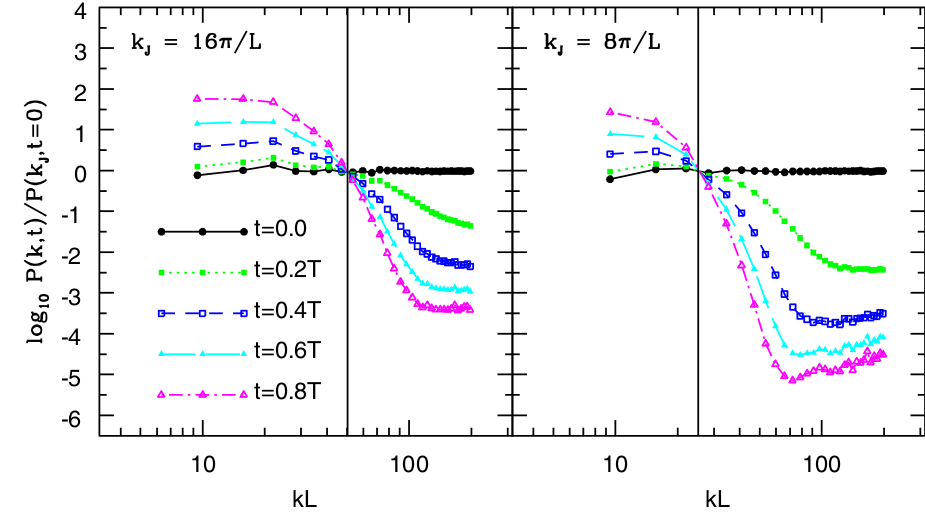
\includegraphics[scale= 0.35]{toReproduceSpectrum.png}
  \caption{Gráfica a reproducir. Note que el tiempo máximo es simplemente 0.8$T$. Imagen tomada de \cite{2013ApJ...762..116Y}}
  \label{fig: toReproduceSpectrum}
\end{figure}
Sin embargo, este test se corrió originalmente para un espacio de fase 6D, por lo que usó $N = 64$. Se hará el test tanto con $N = 64$, como con $N=2048$.


\subsection{Test con N=64}
Usando $N=64$ de resolución tanto para el eje espacial como el de velocidad, junto con $k_j = 8\pi$, la dispersión de velocidad se vuelve demasiado pequeña para permitir obtener una evolución temporal apreciable. Por lo anterior, usamos $k_j = 2\pi$ y $\sigma^2 = \frac{1}{4\pi}$.
La evolución del espectro de potencias para esta inicialización está en la figura \ref{fig: potencias1}.
No se logra observar el comportamiento esperado. El espectro entero oscila sin tener comportamientos que diferencien las frecuencias mayores a $k_j$ de las menores.
Notando el comportamiento tan diferenciado en la gráfica original (figura \ref{fig: toReproduceSpectrum}), hay algo extraño pasando. 
Grafiqué también la evolución temporal del segundo coeficiente de Fourier (figura \ref{fig: coef1}).
Este debería crecer y luego oscilar alrededor de un máximo como en el test de invarianza Galileana. 


\begin{figure}[H]
  \centering
   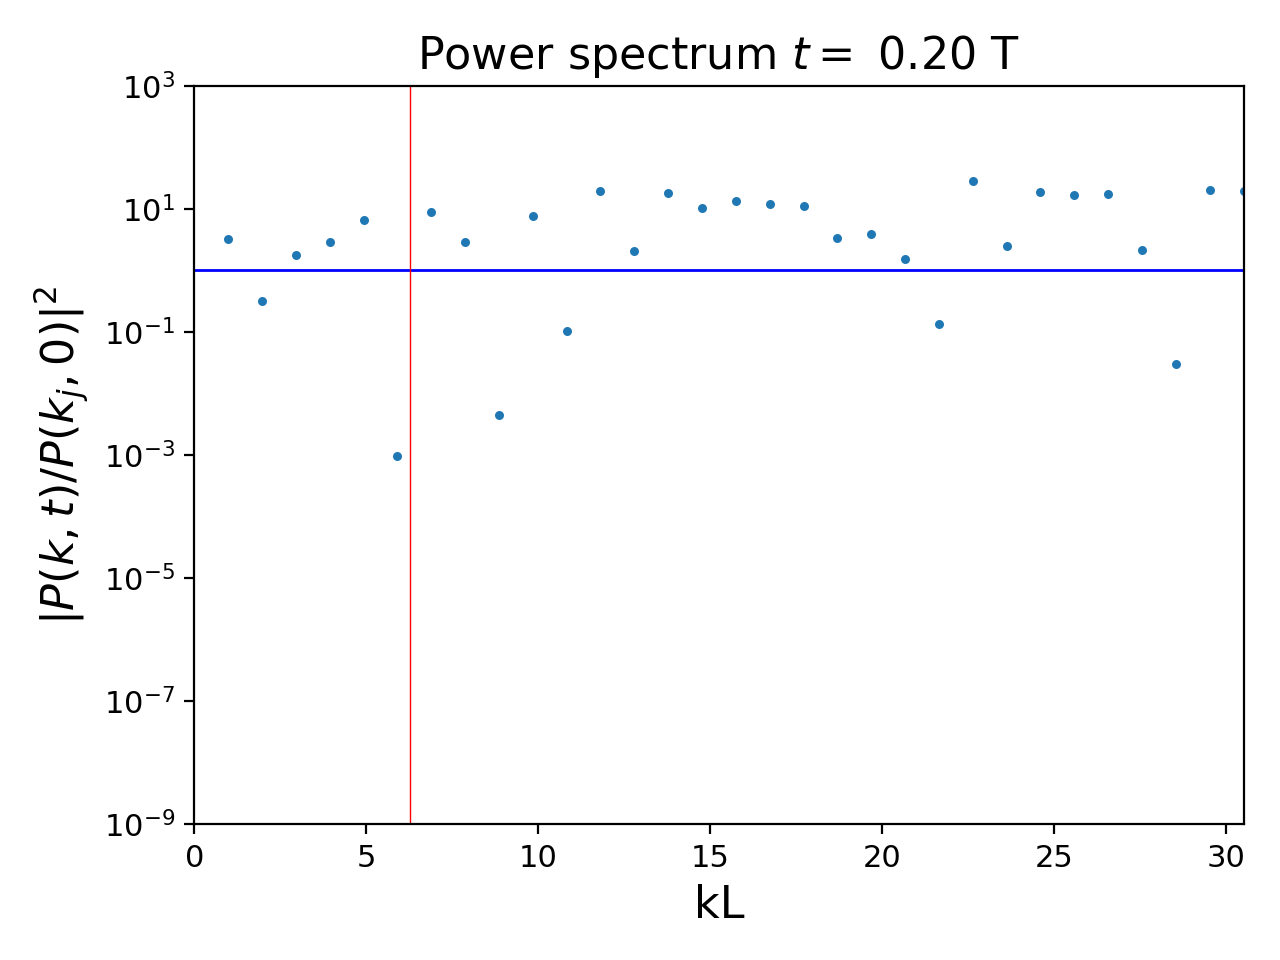
\includegraphics[scale= 0.5]{1powerSeries8.png}
   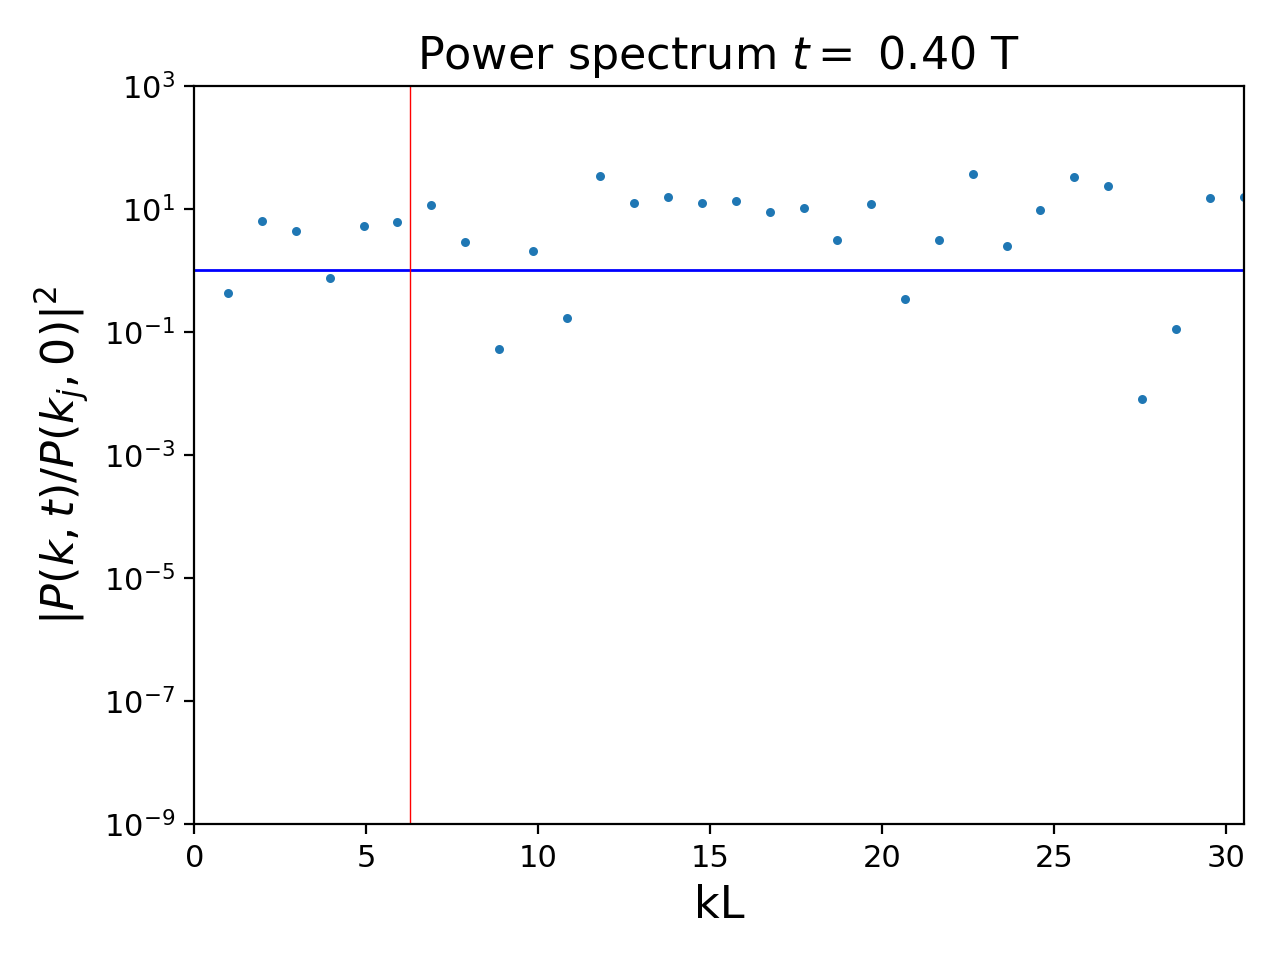
\includegraphics[scale= 0.5]{1powerSeries16.png}
   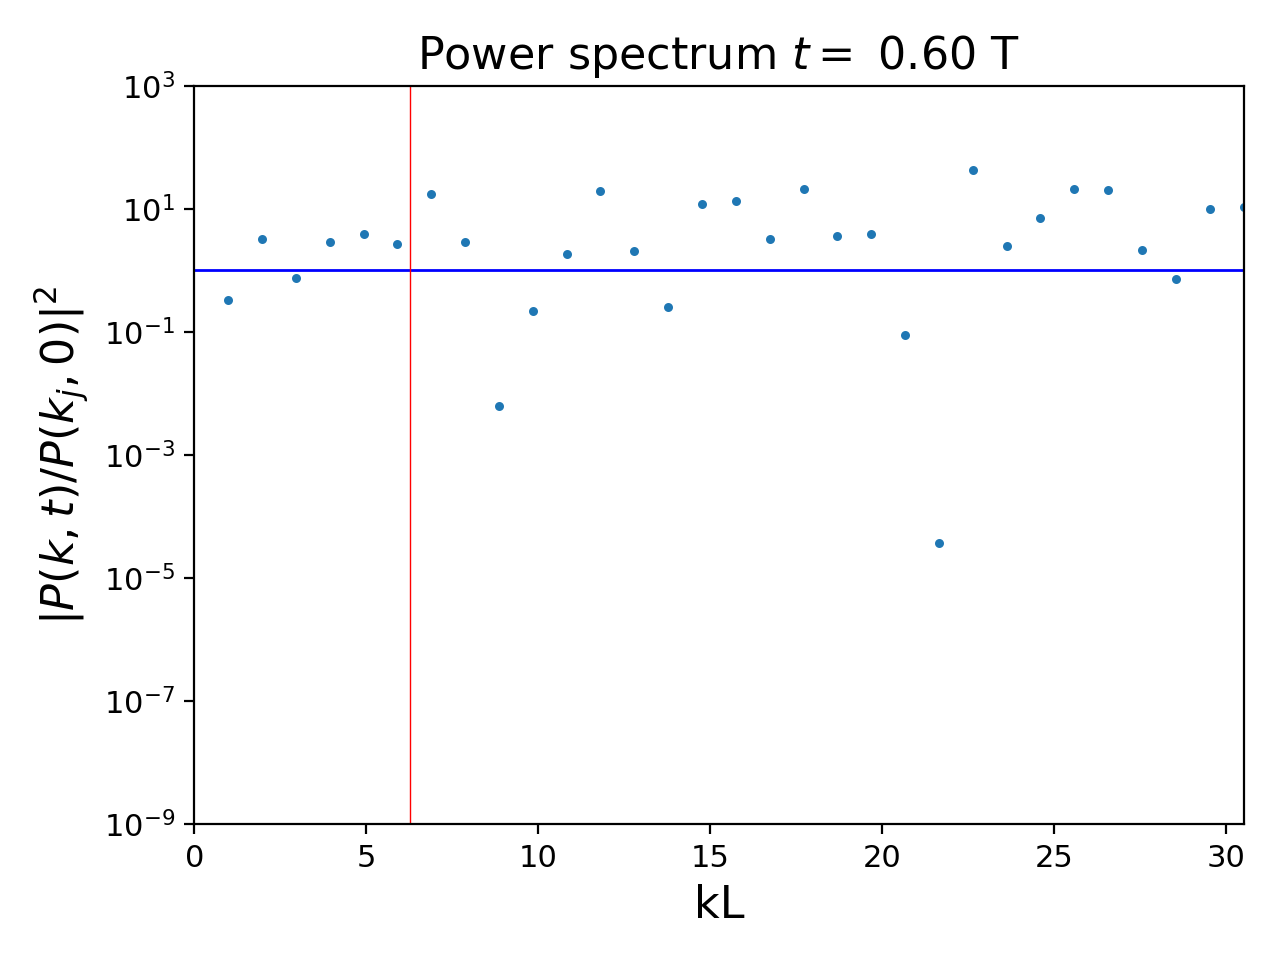
\includegraphics[scale= 0.5]{1powerSeries24.png}
   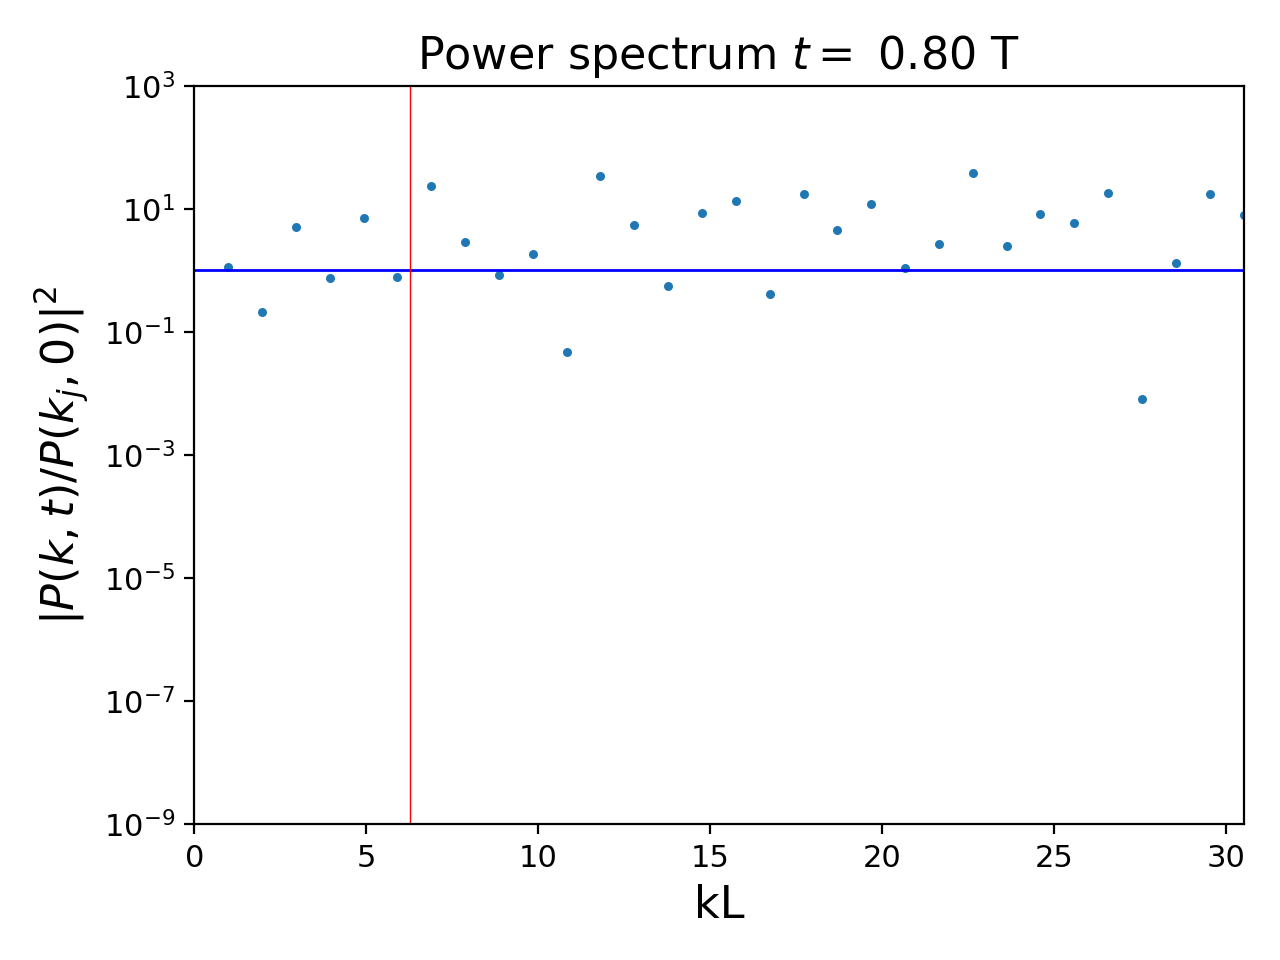
\includegraphics[scale= 0.5]{1powerSeries32.png}
  \caption{Evolución del espectro de potencias para $k_j = 2\pi$  y $\sigma^2 = \frac{1}{4\pi}$ en los mismos tiempos del test del Paper. No se observa el comportamiento esperado. La línea azul señala y = 1, y la línea roja señala la ubicación de $k_j$.}
  \label{fig: potencias1}
\end{figure}

\begin{figure}[H]
  \centering
   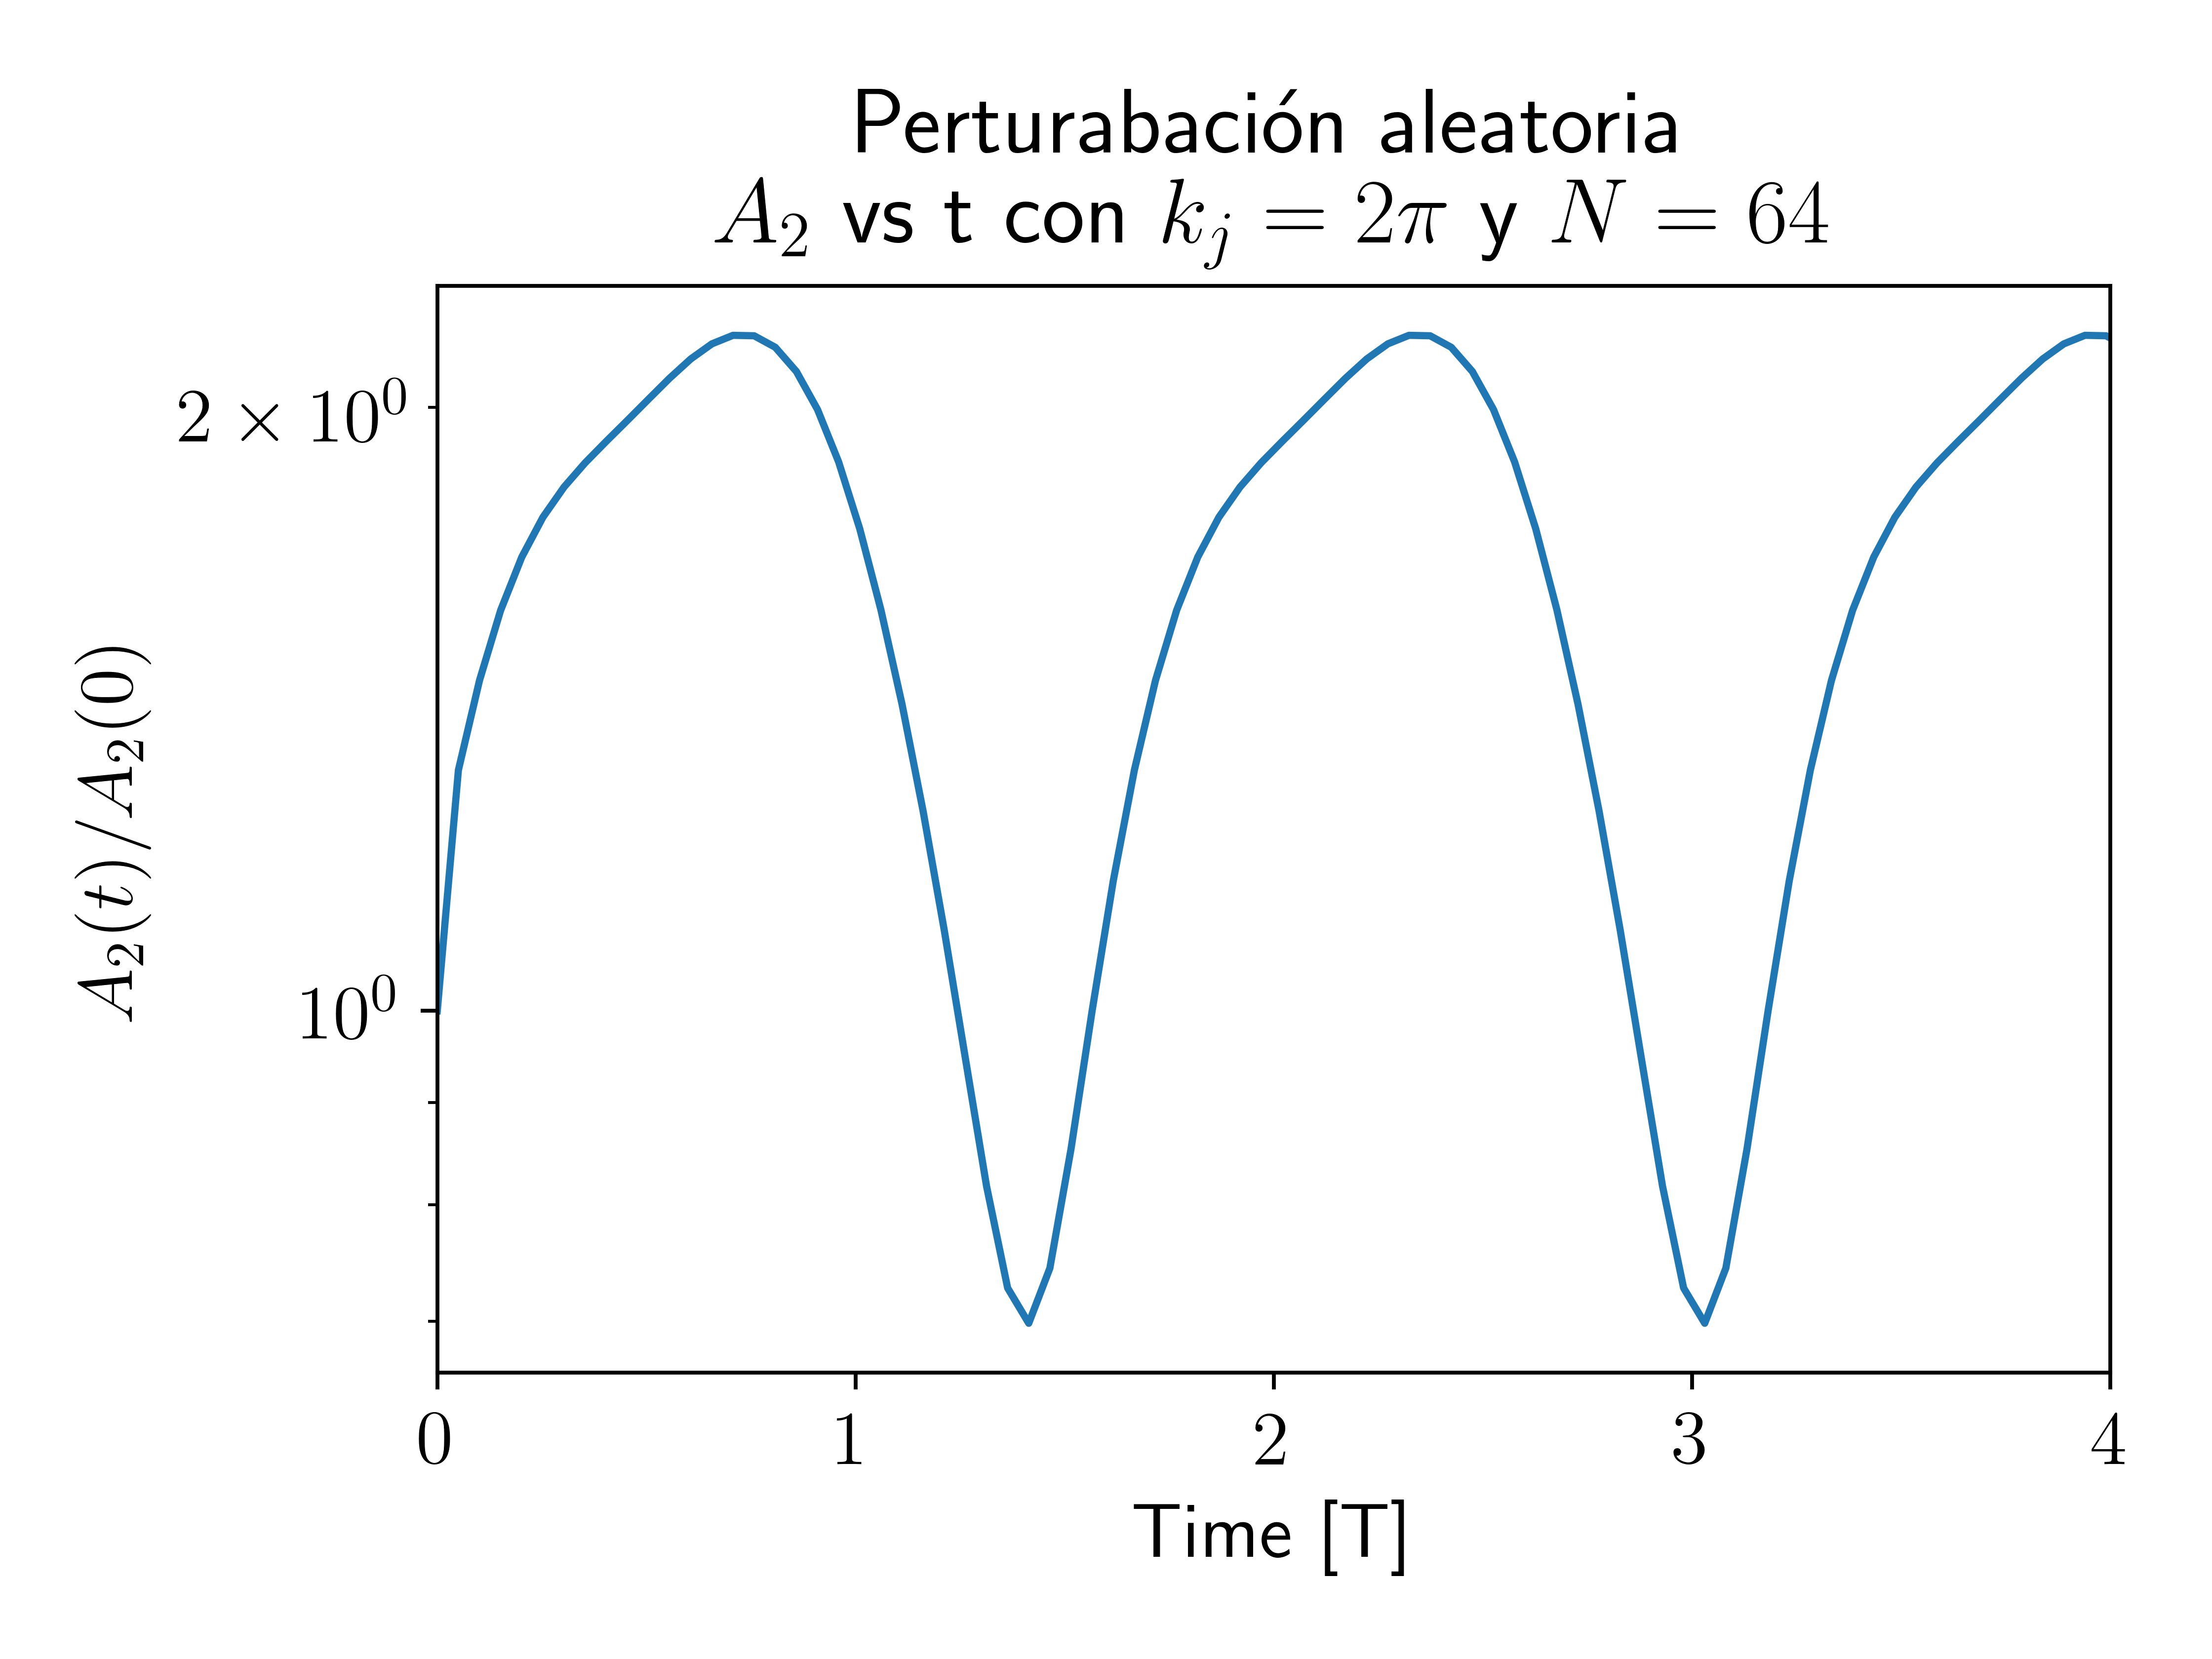
\includegraphics[scale= 0.6]{1Jeans2Coef.png}
  \caption{Evolución del segundo coeficiente de Fourier para la misma inicialización de la gráfica anterior (\ref{fig: potencias1}).}
  \label{fig: coef1}
\end{figure}

El Paper especifica que con los valores usados por ellos la dispersión estará dada por $\sigma = 9\Delta v$. No dan mayor explicación de por qué ese valor. A continuación se presenta la evolución temporal del espectro de potencias (figura \ref{fig: potencias2}) y del segundo coeficiente de Fourier (figura \ref{fig: coef2}).
Una vez más no se obtuvo el comportamiento esperado pues no hay diferenciación entre los $k$ menores a $k_j$ y los mayores.
La evolución temporal del segundo coeficienta de nuevo sigue un comportamiento periódico en vez de oscilar cerca a un máximo.
Se repitió este test con $k_j = 8\pi$ y se obtuvo cualitativamente los mismos resultados.


\begin{figure}[H]
  \centering
   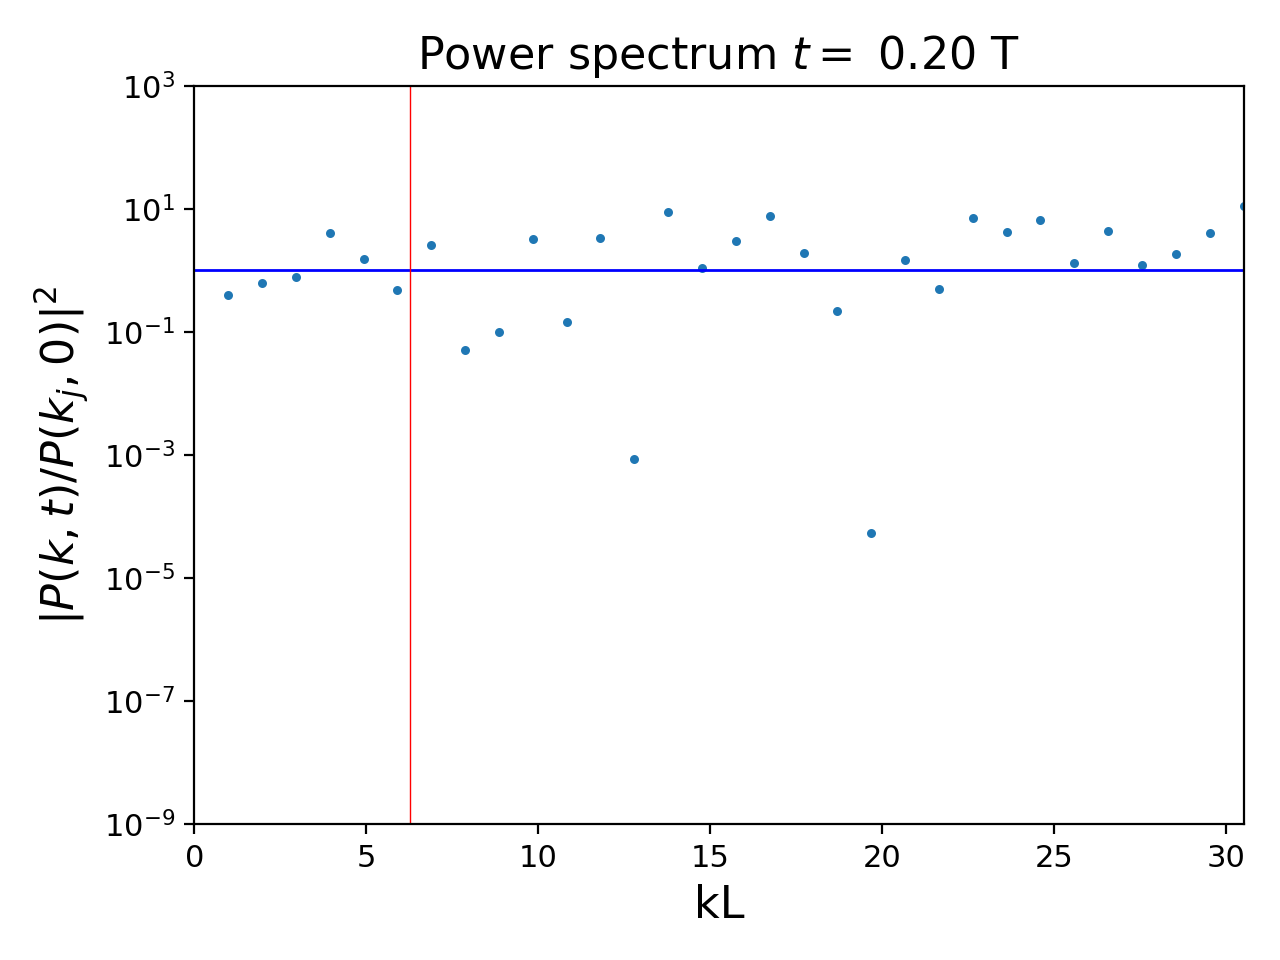
\includegraphics[scale= 0.5]{2powerSeries8.png}
   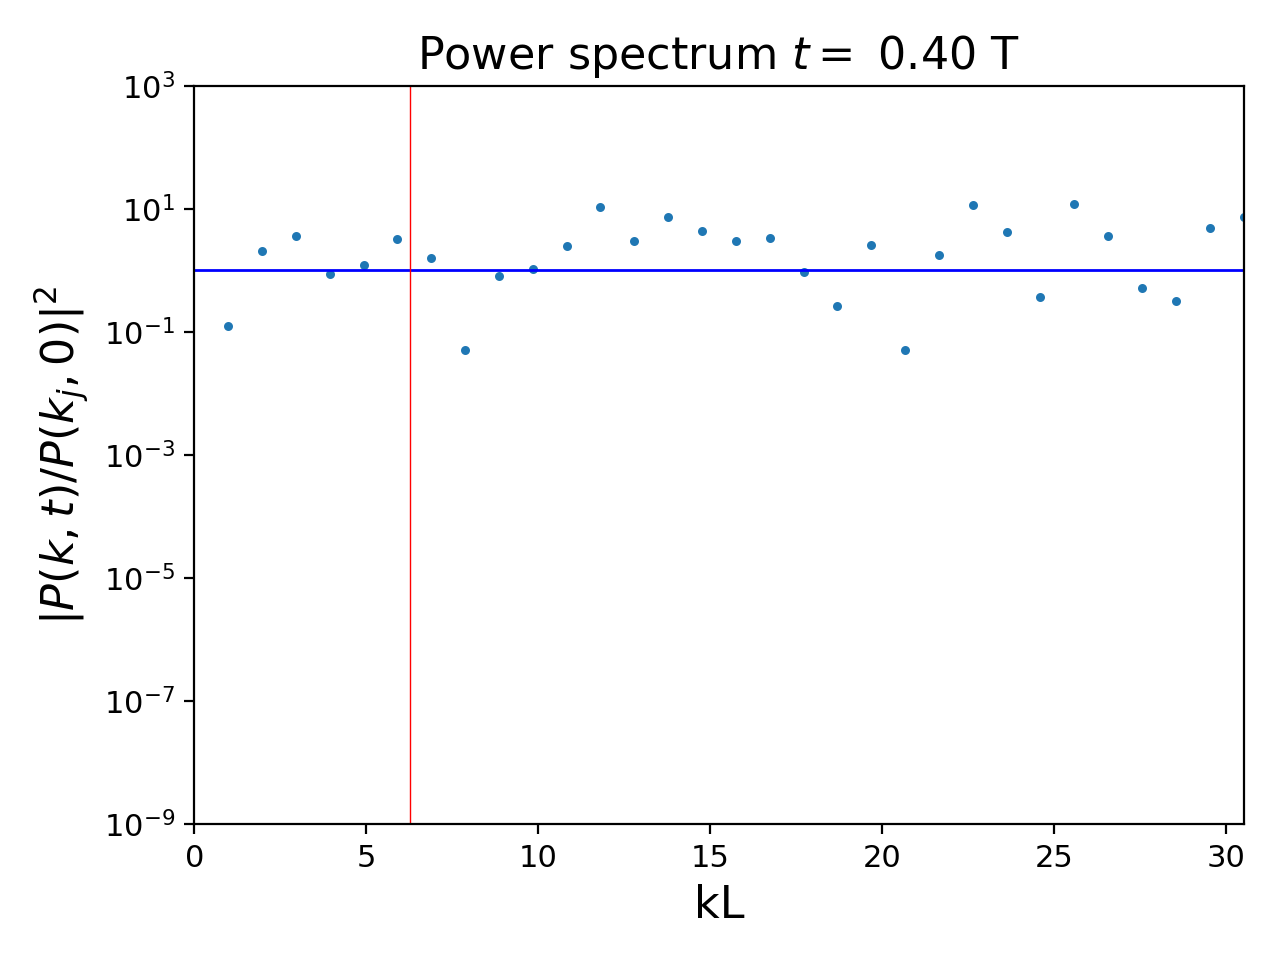
\includegraphics[scale= 0.5]{2powerSeries16.png}
   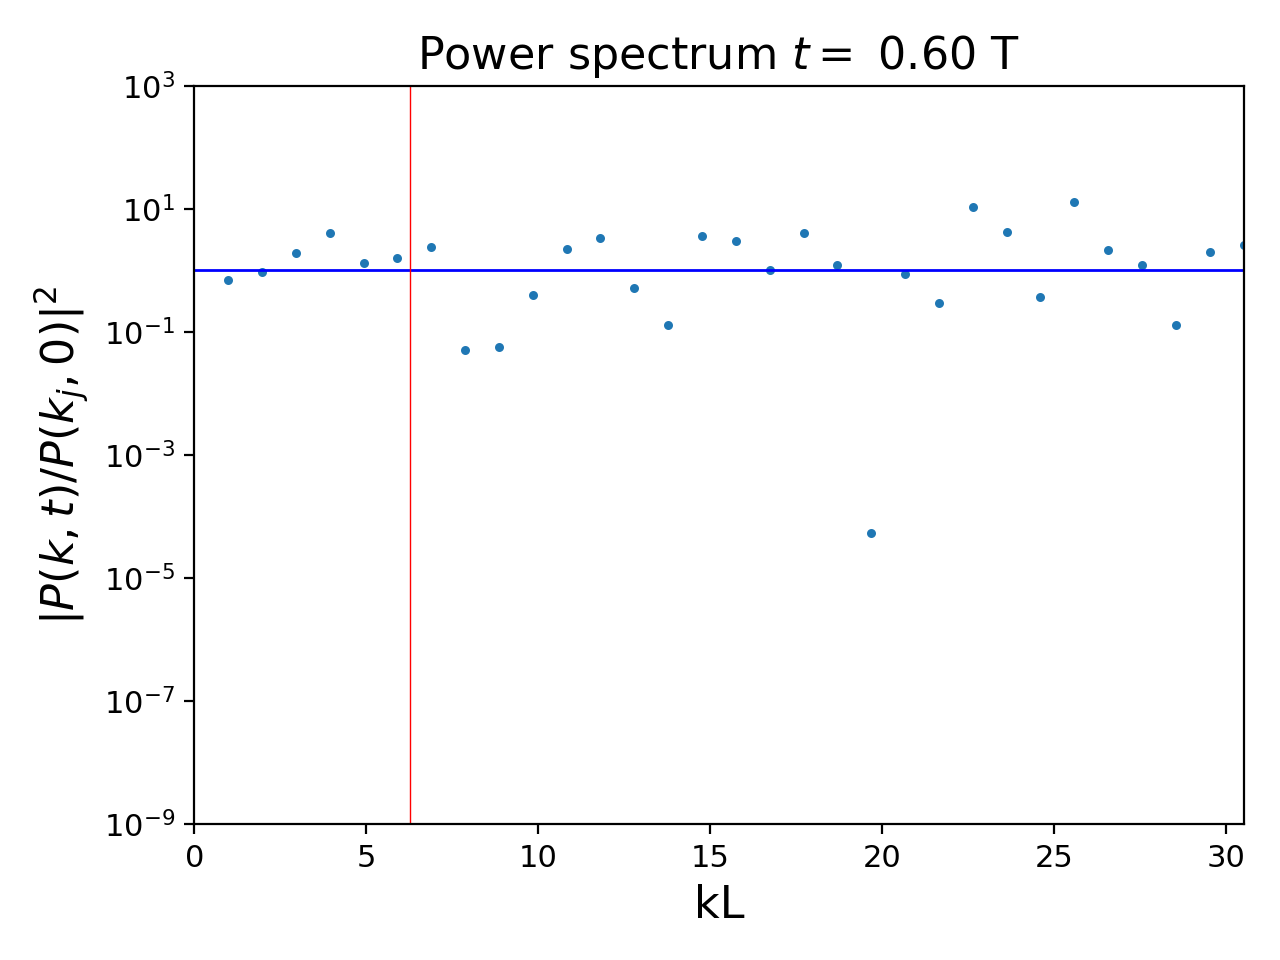
\includegraphics[scale= 0.5]{2powerSeries24.png}
   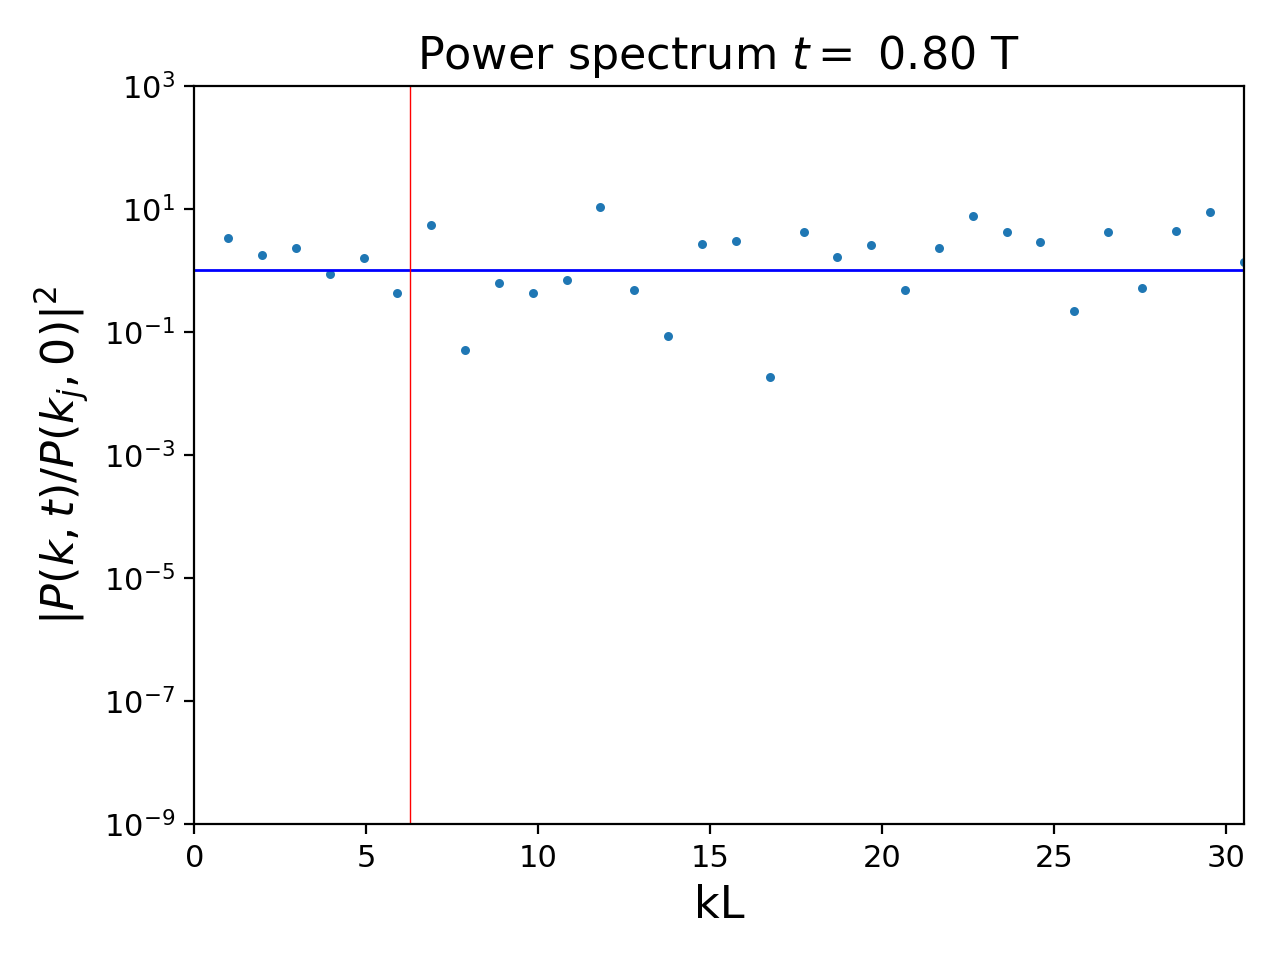
\includegraphics[scale= 0.5]{2powerSeries32.png}
  \caption{Evolución del espectro de potencias para $k_j = 2\pi$  y $\sigma^2 = (9\Delta v)^2$ en los mismos tiempos del test del Paper. No se observa el comportamiento esperado. }
  \label{fig: potencias2}
\end{figure}

\begin{figure}[H]
  \centering
   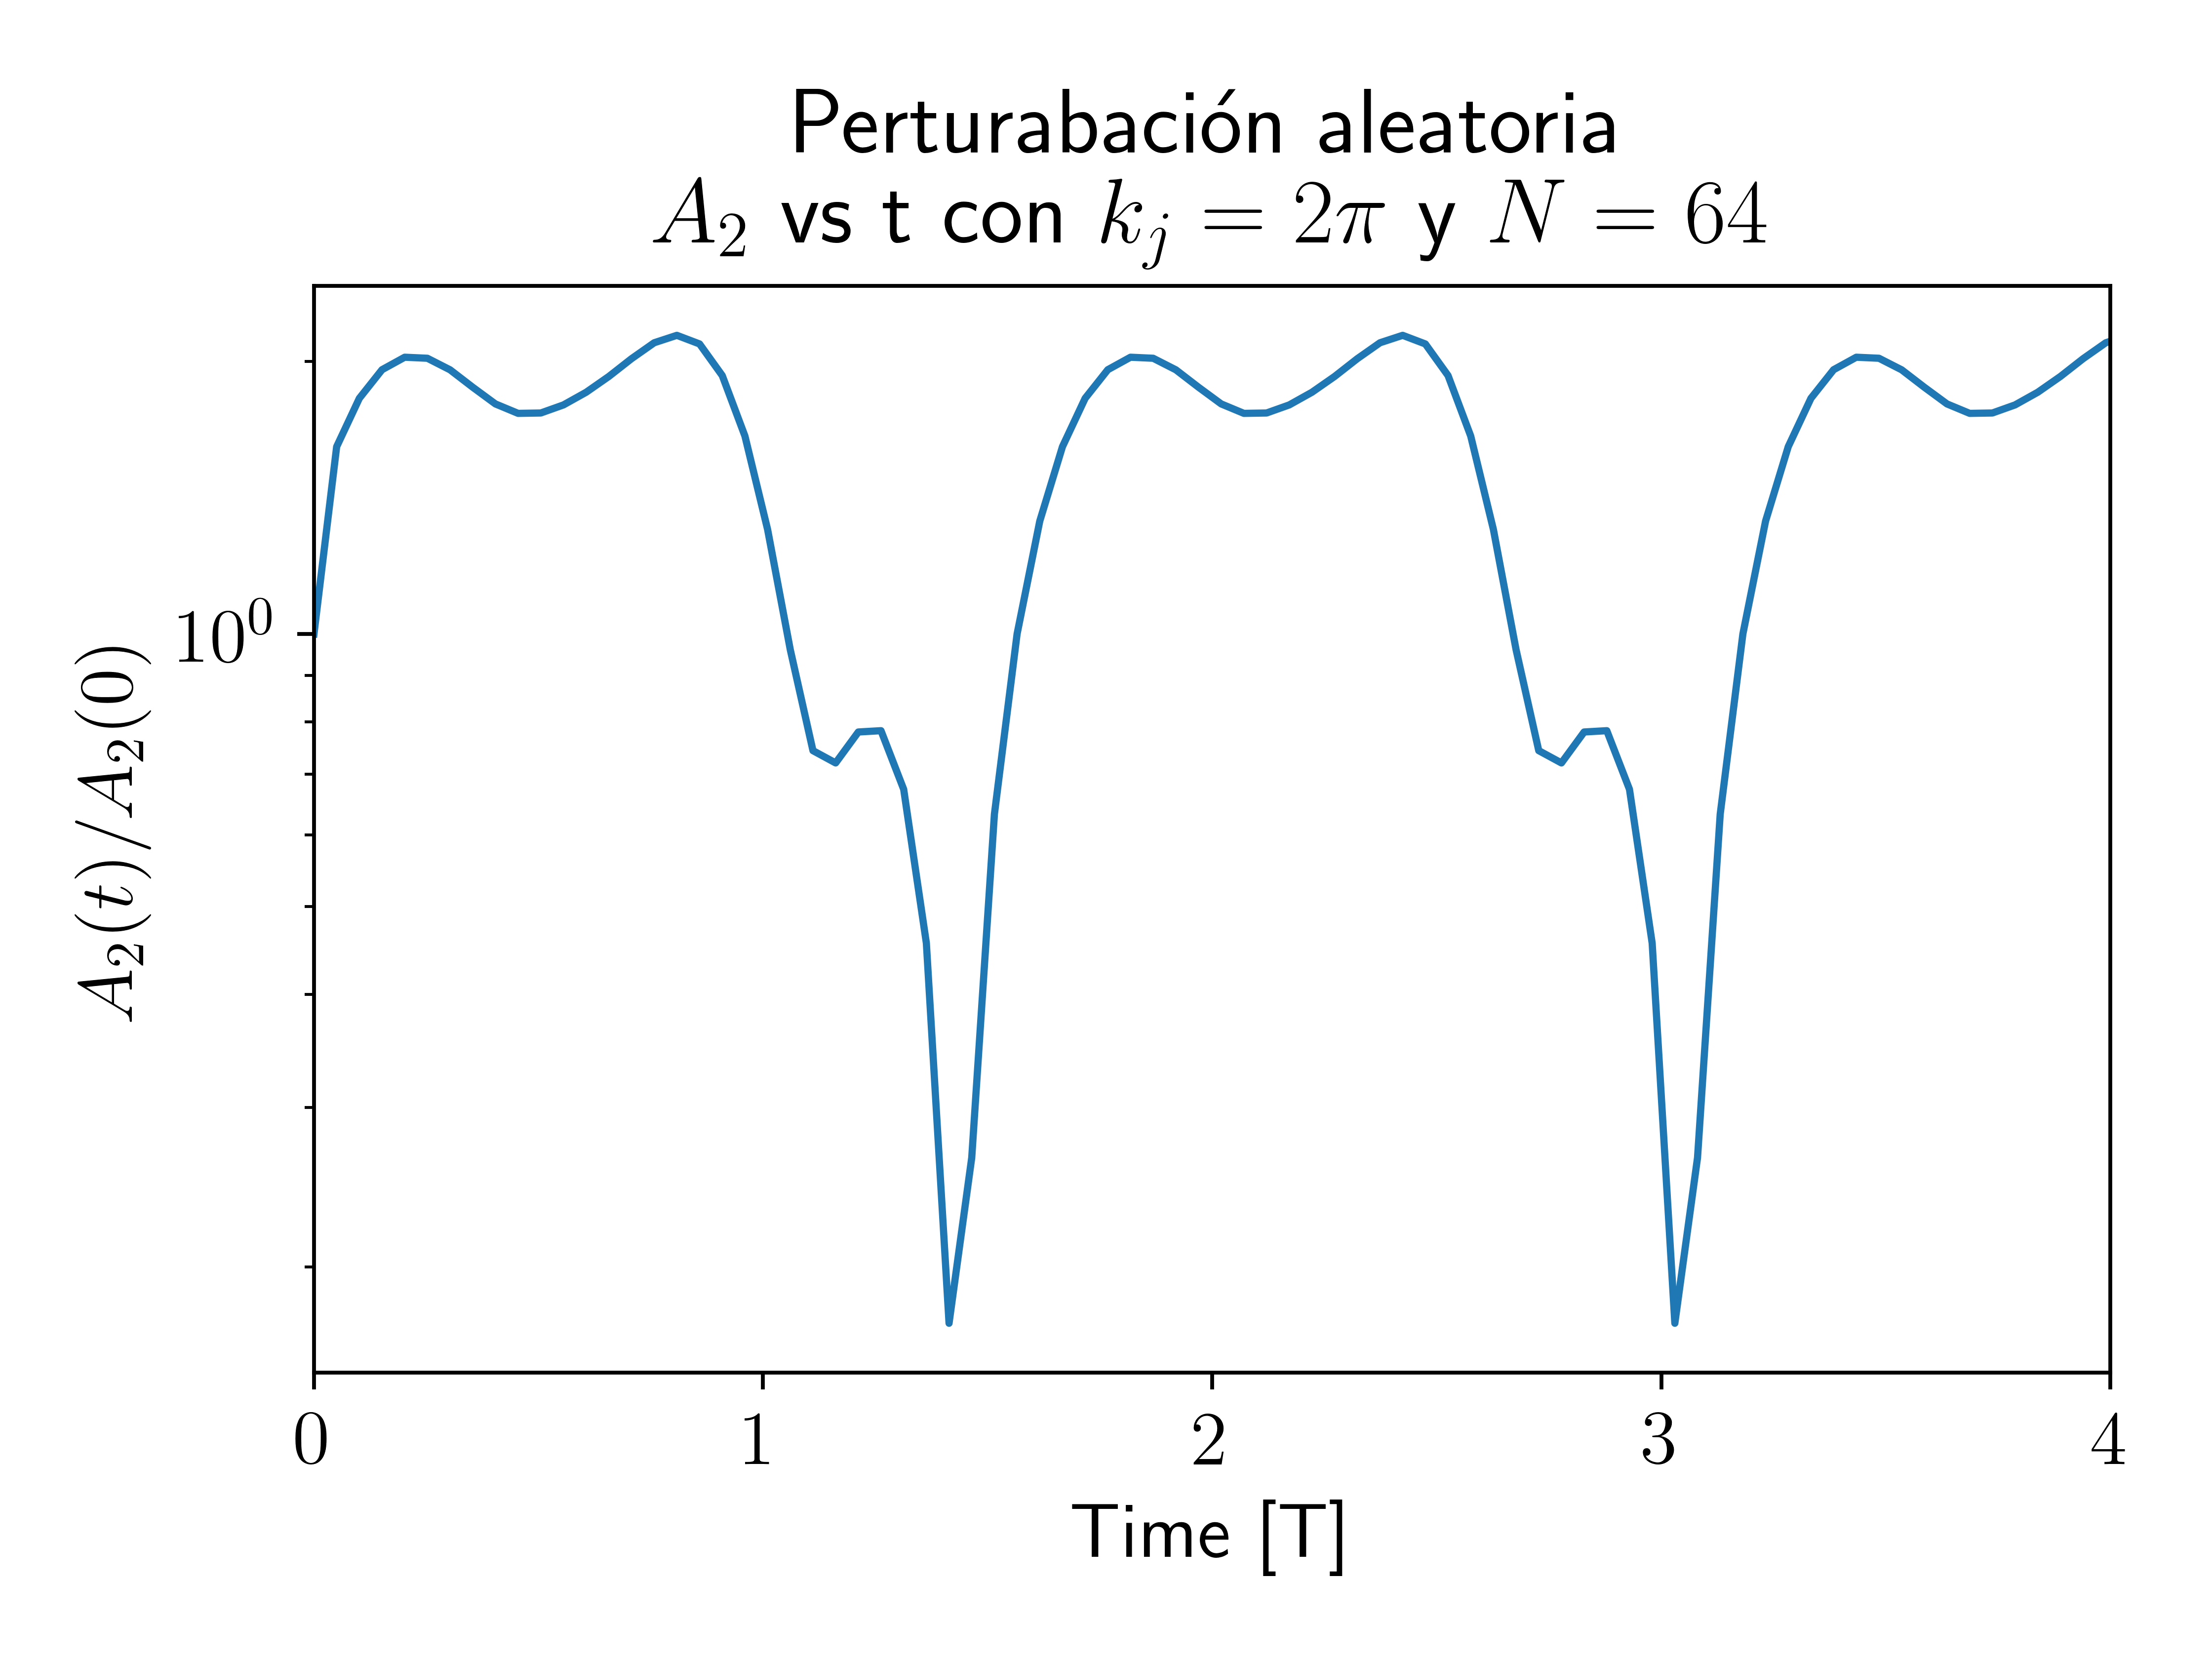
\includegraphics[scale= 0.6]{2Jeans2Coef.png}
  \caption{Evolución del segundo coeficiente de Fourier para la misma inicialización de la gráfica anterior (\ref{fig: potencias1}).}
  \label{fig: coef1}
\end{figure}

\subsection{Test con N = 2048}
Se repitieron los test de la parte anterior con $N = 2048$.
Se presentarán los resultados en el mismo orden.


\bibliographystyle{unsrt} % estilo de las referencias 
\bibliography{bibTes.bib} %archivo con los datos de los artículos citados


%\bibliography{mybib.bib} %archivo con los datos de los artículos citados

% Forma Manual de hacer las referencias
% Se escribe todo a mano...
% Descomentar y jugar

%\begin{thebibliography}{99}
%\bibitem{Narasimhan1993}Narasimhan, M.N.L., (1993), \textit{Principles of
%Continuum Mechanics}, (John Willey, New York) p. 510.

%\bibitem{Demianski1985}Demia\'{n}ski M., (1985), \textit{Relativistic
%Astrophysics,} in International Series in Natural Philosophy, Vol 110, Edited
%by \textit{D. Ter Haar}, (Pergamon Press, Oxford).
%\end{thebibliography}


%Fin del documento
\end{document}


Así mismo, el factor de calidad $Q$ está dado por:
\begin{equation}
Q = \frac{1}{R} \sqrt\frac{L}{C}
\end{equation}
Por lo tanto, el valor del factor de calidad

%Todo lo que escriba aquí será ignorado, aunque no fuera un comentario...
\begin{table}[h!]
\centering
\begin{tabular}{|l|l|l|}
\hline
2 cm   & 4 cm   & 8 cm   \\ \hline
175,77 & 129,77 & 88,77  \\ \hline
223,77 & 129,77 & 114,77 \\ \hline
219,77 & 134,77 & 77,77  \\ \hline
190,77 & 120,77 & 83,77  \\ \hline
\end{tabular}
\caption{Número de colisiones a diferentes distancias en cinco minutos.}
\label{tiempoFijo}
\end{table}

\begin{figure}[h]
  \centering
   \includegraphics[scale= 0.8]{jairos.png}
  \caption{Gráfica del periodo de la pulsación para diferentes razones entre las frecuencias naturales utilizando una pesa de 200g. Es de resaltar que el pico no está centrado en 1 pero está bastante cerca. Esto probablemente se debe a errores a la hora de medir la longitud de los péndulos.}
  \label{fig: cobre}
\end{figure}
